
%(BEGIN_QUESTION)
% Copyright 2012, Tony R. Kuphaldt, released under the Creative Commons Attribution License (v 1.0)
% This means you may do almost anything with this work of mine, so long as you give me proper credit

Large electric power distribution transformers are filled with a special high-dielectric oil that helps transfer heat from the transformer core to cooling tubes, as well as displace moisture from the internal volume of the device.  One of the important operational parameters of such transformers is the temperature of this oil.

A special-purpose protection device called a {\it thermal overload protective relay} (ANSI/IEEE code number 49) uses an RTD sensor to detect the transformer's temperature, then energizes the circuit breaker's ``trip'' coil (causing the breaker to open its contacts) if ever this temperature exceeds a certain pre-set value.  A basic schematic diagram shows how this relay device triggers the circuit breaker to trip if necessary to protect the transformer against over-temperature:

$$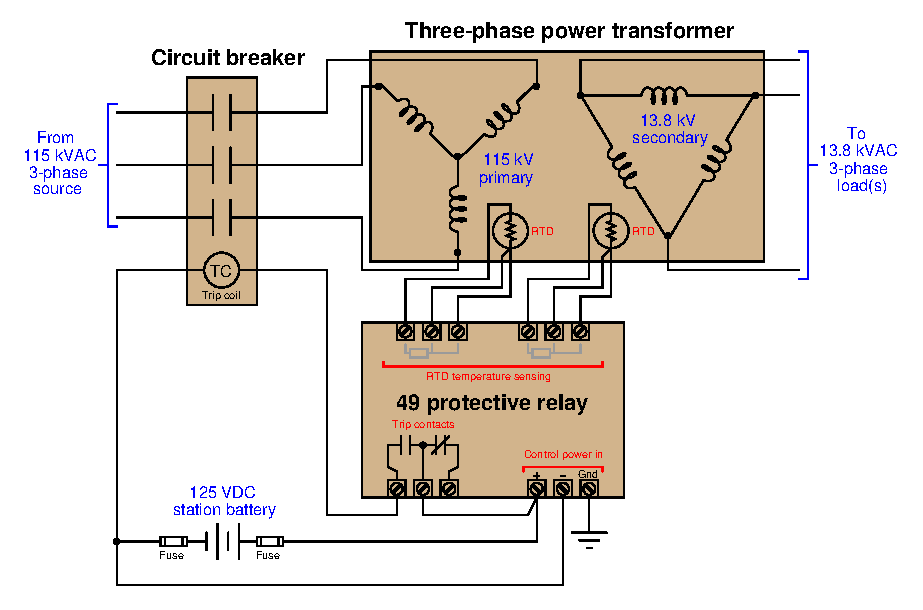
\includegraphics[width=15.5cm]{i02032x01.eps}$$

Identify how you would perform an ``As-Found'' test on this protective relay to ensure it would act to trip the circuit breaker in the event the transformer got too hot, without actually tripping the breaker.  In other words, devise a ``live'' test of the protective relay that does not actually interrupt power to the transformer during the test.  Assume the transformer's trip temperature setting is 60 degrees Celsius, and that the formula relating RTD resistance with temperature is as follows:

$$R = 100 [ 1 + 0.00385 T ]$$

Be sure to specify any temporary changes you would make to the wiring in order to safely conduct your ``As-Found'' test, and describe the step-by-step procedure as though you were giving instuctions to another technician to perform the test instead of you.

\vskip 20pt \vbox{\hrule \hbox{\strut \vrule{} {\bf Suggestions for Socratic discussion} \vrule} \hrule}

\begin{itemize}
\item{} The specific {\it sequence} in which you perform the steps of your As-Found calibration test is every bit as important as the steps themselves!  Identify where an improper sequence of otherwise proper steps would cause things to go wrong during the test.
\item{} For those who have studied RTD sensors before, identify the proper amount of resistance equivalent to 60 degrees Celsius from an {\it RTD table} rather than using the given formula.
\end{itemize}

\underbar{file i02032}
%(END_QUESTION)





%(BEGIN_ANSWER)

There is a {\it lot} to consider when planning the As-Found calibration test.  What I am looking for here is a complete step-by-step procedure describing a safe and logical way to conduct the test without causing the circuit breaker to trip.

%(END_ANSWER)





%(BEGIN_NOTES)

Calculating the proper RTD resistance for 60 degrees Celsius:

$$R = 100 [1 + 0.00385 T]$$

$$R = 100 [1 + (0.00385)(60)]$$

$$R = 100 [1 + 0.231]$$

$$R = 100 [1.231]$$

$$R = 123.1 \> \Omega$$

\vskip 10pt

The very first step to perform is to disable the relay's ability to trip the circuit breaker.  Disconnecting the wire between the relay and the breaker's trip coil would suffice, taking care to perform this disconnection in such a way as to avoid shock hazard.  Re-enabling the relay's ability to trip the breaker should be the very last step.  

Given that this will be a {\it high} temperature trip function, the calibration test should be done with the resistance {\it increasing} rather than decreasing.  In other words, the relay should issue a trip command (as verified by an ohmmeter) at 123.1 $\Omega$ {\it rising}.

%INDEX% Protective relay: transformer thermal overload (49)

%(END_NOTES)


